\documentclass{article}\usepackage[]{graphicx}\usepackage[]{color}

\usepackage{alltt}
\usepackage{float}
\usepackage{graphicx}
\usepackage{tabularx}
\usepackage{siunitx}
\usepackage{amssymb} % for math symbols
\usepackage{amsmath} % for aligning equations
\usepackage{textcomp}
\usepackage{booktabs}
\usepackage{mdframed}
\usepackage{natbib}
\usepackage[colorinlistoftodos]{todonotes} % to make comments on the margin
\usepackage[small]{caption}
\setlength{\captionmargin}{30pt}
\setlength{\abovecaptionskip}{0pt}
\setlength{\belowcaptionskip}{10pt}
\topmargin -1.5cm        
\oddsidemargin -0.04cm   
\evensidemargin -0.04cm
\textwidth 16.59cm
\textheight 21.94cm 
%\pagestyle{empty} %comment if want page numbers
\parskip 7.2pt
\renewcommand{\baselinestretch}{1.5}
\parindent 0pt
%\usepackage{lineno}
%\linenumbers

%% R Script

\title{Woody plant phenological responses are strongly associated with key functional traits- Outline}

\begin{document}

\maketitle

\noindent Authors:\\
The Wolkovich Lab in 2021 $^{1,2,3,4}$
\vspace{2ex}\\
\emph{Author affiliations:}\\
$^{1}$Forest \& Conservation Sciences, Faculty of Forestry, University of British Columbia, 2424 Main Mall, Vancouver, BC V6T 1Z4;\\
$^{2}$Arnold Arboretum of Harvard University, 1300 Centre Street, Boston, Massachusetts, USA;\\
$^{3}$Organismic \& Evolutionary Biology, Harvard University, 26 Oxford Street, Cambridge, Massachusetts, USA;\\
$^{4}$Edificio Ciencias, Campus Universitario 28805 Alcalá de Henares, Madrid, Spain\\
 

\vspace{2ex}
$^*$Corresponding author: deirdre.loughnan@alumni.ubc.ca\\
\renewcommand{\thetable}{\arabic{table}}
\renewcommand{\thefigure}{\arabic{figure}}
\renewcommand{\labelitemi}{$-$}
\setkeys{Gin}{width=0.8\textwidth}

Climate change is altering the timing of species phenologies, with changes in temporal niches reshaping ecological communities and interactions between species. In temperate systems, the observed advances in plant phenological events, such as budburst, leafout, and flowering times, are associated with changes in seasonal temperatures, particularly warming winter and spring conditions \citep{Menzel2006,Fitter2002}. But despite this strong general trend, phenological responses vary across species and geographically, and we have yet to fully understand the underlying mechanisms driving observed differences \citep{Chuine2010,Morin2009}. As the effects of climate change become more pronounced, understanding these relationships is of increasing importance if we are to predict and preserve the diversity and services found in temperate forest ecosystems. %The relationships between environmental cues and phenological events define for example, the duration of the growing season, the trajectory of community assembly, species ranges, and ecosystem services \citep{Cleland2007,Lopez2008,Chuine2010}, ultimately shaping and mitigating the impact of climate change on forest communities.

While we have yet to identify all drivers of selection on phenologies, considerable work has shown the importance of three abiotic cues -- chilling, forcing, and photoperiod -- as the primary drivers of budburst and leafout in temperate deciduous species \citep{Basler2014,Chuine2016, Harrington2016,Flynn2018}. For budburst to occur, species must experience extended period of cold temperatures to break dormancy \citep{Cooke2012}, where species with higher chill requirements budburst later in the season. Spring forcing temperatures, or the temperatures needed to cue species to initiate growth after dormancy release, are also changing as temperatures warm and the timing at which suitable temperature thresholds are met occur earlier within the season (citation). Photoperiod cues can also determine a species ability to initiate growth \citep{Basler2014,Zohner2020}. Species with strong photoperiod requirements are, however, expected to be more constrained in their ability to track changes in temperature and may face fitness costs and novel species interactions as a result \citep{Guy2014, others?}. Previous studies support the general trend of advancing budburst in response to each cue, but with considerable variation in the relative importance of different cues across species \citep{Chuine2016,Flynn2018}. Some woody plant species, for example, require less forcing to budburst after experiencing a cool winter with more chilling, while also having the ability to compensate for low chilling with high forcing conditions or longer photoperiods \citep{Laube2014,Harrington2015,Flynn2018,Caffarra2011,Basler2014,Zohner2016}. Evidence for the role of photoperiod is largely species specific  \citep{Heide1993, Basler2014, Singh2017, Zohner2016}, with few studies testing for its importance across species in a community (but see  \cite{Flynn2018}). Species that are less dependent on photoperiod cues and able to track trends in temperatures may benefit from greater intra-annual phenotypic plasticity resulting in greater fitness outcomes under increasingly variable climates (citation?). Despite the insights that identifying these proximate drivers have provided, we still lack a generalizable and mechanistic understanding of why species and populations differ in their cue use that. Further insight on this topic is needed to predict future changes in species sensitivities and community structure.\\

In our efforts to understand variation in spring phenological timing, researchers have tested several potential mechanisms to identify the drivers of species cue responses. Work exploring drivers of intraspecific cue use, for example, has found age or the development stage of woody plants to be important. Younger life stages, including both seedlings and younger understory trees, budburst earlier than mature individuals in the canopy \citep{Vitasse2013,Seiwa1991}. These trends reflect both differences in the temperature sensitivities across life stages and effects of ontogenic changes as trees mature \citep{Vitasse2013,Seiwa1991}. Interspecific differences in cues, however, have been studied in relation to species' phylogenetic relatedness. Work on this topic has found strong evidence for events like flowering-time and budburst to be consistent within taxonomic families, suggesting conservatism in the genetic and physiological mechanisms that determine species phenologies \citep{Kochmer1986,Davies2013,Gougherty2018}. Studies of woody plant phenologies across species ranges have also highlighted the importance of local adaptations, with the presence of gradients in phenological responses and presumably cue use at northern range limits \citep{Lechowicz1984,Chuine2001,Chuine2010}. In temperate systems for example, greater temperature variation in North America was associated with higher chilling requirements and more conservative phenological responses \citep{Zohner2017}.  Studies testing for trends in cues responses across species latitudinal ranges have also observed stronger responses to photoperiod cues at lower latitudes \citep{Zohner2016}. Exploring these potential drivers of plant phenologies have illustrated the nuanced nature of phenology in shaping diverse communities, but they are still limited in the degree to which they explain the variation we observe across species and ecosystems.\\

Taking a functional trait approach to phenological research could help explain the variation in cue use across species and geographically \citep{Flynn2018,Osada2017}. Early work on functional traits used trait data from diverse global assemblages of deciduous plants to identify associations between traits, common growth strategies, and different niche space \citep{Westoby1998,Wright2004,Chave2009}. The resulting leaf-height-seed scheme and the more extensive leaf economic spectrum found direct associations between several trait values and gradients in species growth rates and competitive abilities \citep{Westoby1998,Wright2004,Diaz2016,Chave2009,Funk2016}. While reproductive phenological traits have been identified as ecologically important for many years \citep{Weiher1999, Laughlin2014}, few studies have explored their role in the larger trait framework. Spring phenological traits, such as budburst and leafout, define the beginning of the growing season and period of photosynthesis, and therefore also have the potential to correlate with established growth strategies. Support for the existence of trade-offs in budburst dates and traits related to growth and resource use have been observed across plant functional groups and habitat types in a handful of studies. For example, several studies have found deciduous woody species with smaller vessel diameters and diffuse or semi-ring-porous xylem structures to leaf out earlier than species with larger vessels, as this anatomy reduces the risk of embolism during freezing events  \citep{Panchen2014, Lechowicz1984}. In testing relationships between budburst and leaf traits of deciduous tree species in Japan, \citep{Osada2017} found positive correlations between budburst date and leaf area, leaf mass, and nitrogen content by both mass and area, while \citep{Sun2006} found deciduous species with high leaf mass per area (a trait that is the inverse of specific leaf area) to budburst earlier in deciduous oak forests in eastern China. %Note their prediction is opposite ours 
Variation in leafout can also relate to species heights, both intraspecifically and across functional groups, with shorter individuals or understory species leafing out earlier than taller individuals or canopy species \citep{Seiwa1998, 1999b}. To date, however, research in this area has focused on individuals at local scales, or few traits for a small number of species, limiting our ability to draw more general and causal inferences. There is also a lack of studies linking traits directly to cue sensitivity rather than phenological date. The likely associations between cue sensitivity, phenological events, and growth strategies may allow for more generalizable trends across species and sites, and better account for species variability in key environmental cue use. \\


%Studies of flowering phenology in herbaceous species also find phenology to relate to commonly measured traits, with early germinating species being taller with greater relative growth rates than later germinating species \citep{Sun2011}. 

% Faith commented that the first two sentences below are repetitive 
To date, there have been numerous studies investigating the relationships between climate and functional traits and a wealth of literature on the separate effects of climate cues as drivers of phenology. However, the selective pressures shaping species traits under variable temperatures are also likely to act on species responses to phenological cues and define a species temporal niche. Species with a more acquisitive life-strategy have shorter rates of return on resource investments and the ability to take advantage of the greater abundance of soil nutrients and light early in the growing season. Such species face a lesser cost in initiating phenological events too early, as they can recover from early season damage (cite Cat's paper?). For example, some acquisitive species produce leaves with high leaf nitrogen content and Specific Leaf Area (SLA) and can take advantage of greater light availability by having higher rates of photosynthesis \citep{Wright2004,Pereira2020}, while also limiting the costs of tissue production \citep{Lambers2004, Westoby2006, Herault2011}. Acquisitive-strategy species also invest less in their wood structure, having shorter heights and lower stem densities \citep{Laughlin2010}. Species that budburst earlier in the growing season require less spring forcing and winter chilling, and shorter photoperiods \citep{Flynn2018}, allowing them to grow under less competition for light and soil resources. The suite of traits of acquisitive species contrasts with more conservative life-strategy species that exhibit slower, more competitive growth strategies that benefit from slower rates of return on resource investment and the longer retention of leaf tissue. A greater requirement for cue unit accumulation to trigger phenological events should align with a more conservative life-strategy as such species seek to avoid damage due to premature development.      
 
% Hmmm... is this paragraph still relying heavily on early/late narative?
   
In this study, we test for associations between plant phenological responses to environmental cues and common functional traits. Budburst data for tree species in controlled environmental studies was selected from the Observed Spring Phenology Response in Experimental Environments (OSPREE) database and paired with functional trait data from the TRY and BIEN databases. This data was used to explicitly test for the relative differences in functional traits and the timing of budburst in response to experimental forcing, chilling, and photoperiod cues. Drawing on previous work and the broader trait literature, we predict that species that respond less strongly to chilling, forcing, and photoperiod conditions are more likely to have traits associated with acquisitive growth but low competitiveness, as reflected by high SLA, high leaf nitrogen content per mass (LNC), shorter heights, and lower seed mass. In contrast, species that are more responsive to chilling, forcing and photoperiods will have traits more associated with conservative growth and higher competitive abilities, such as low SLA, low LNC, greater heights and heavier seeds. 


\begin{figure}[h!]
    \centering
 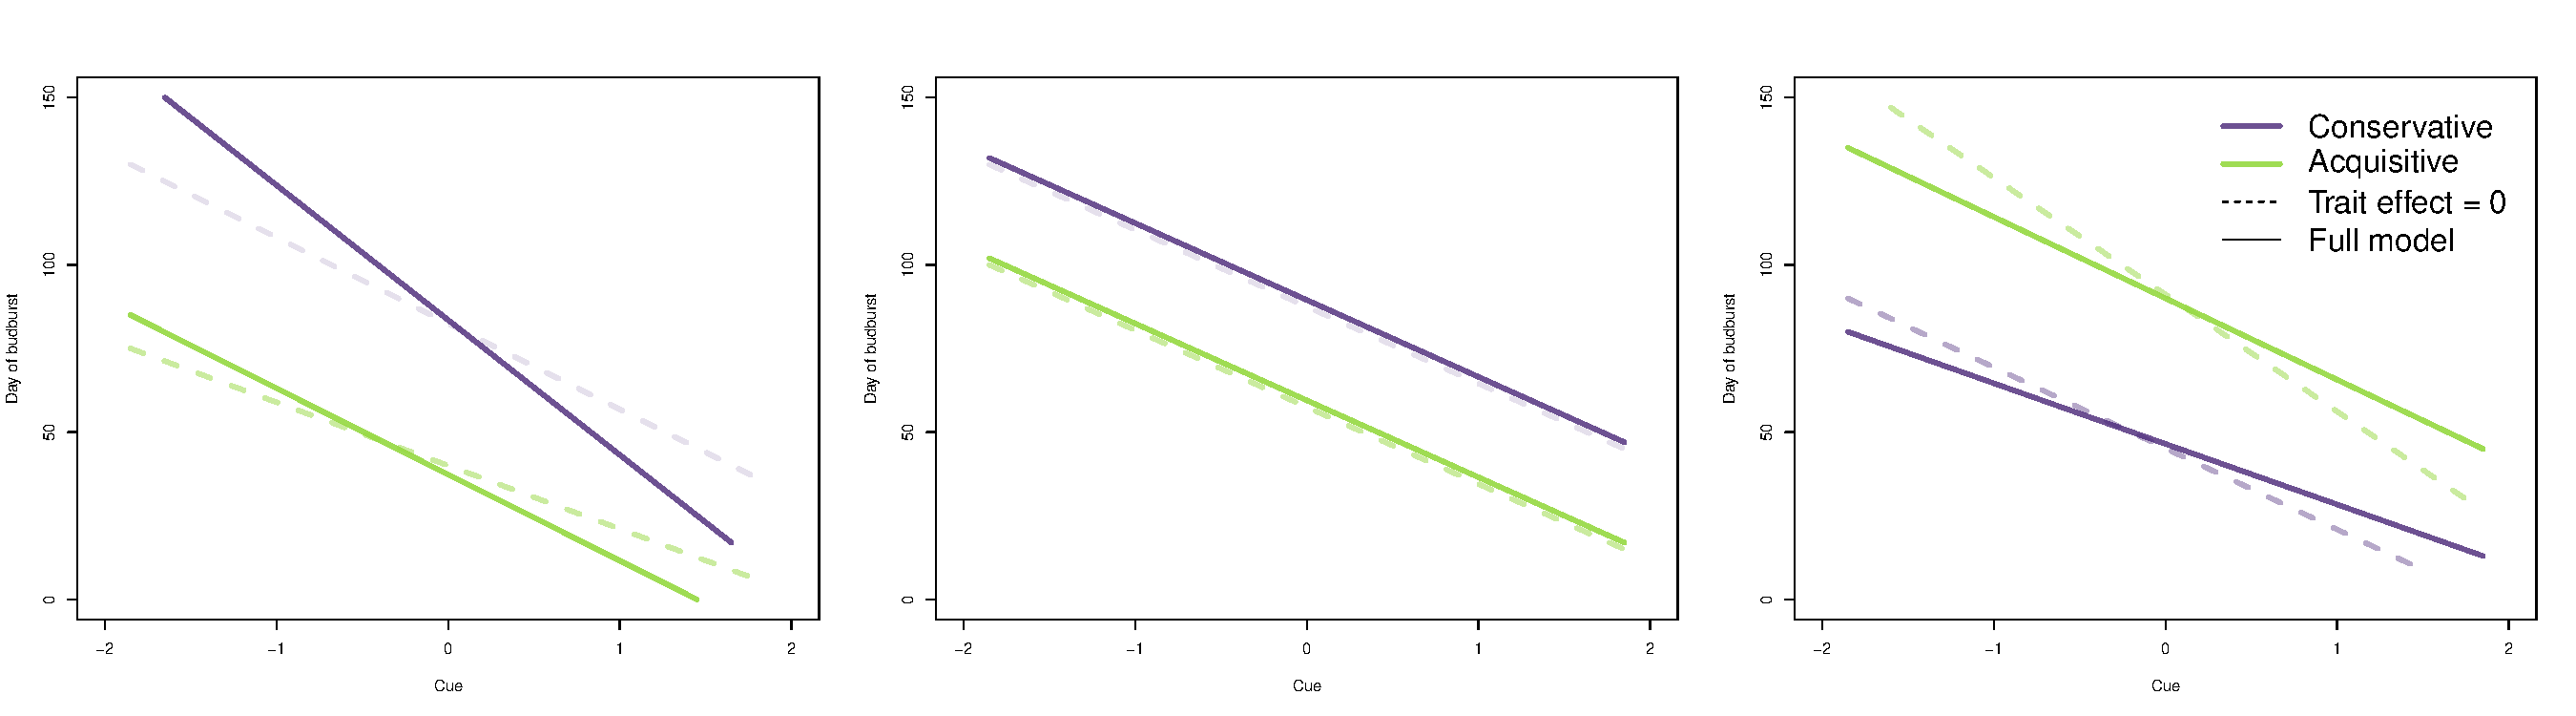
\includegraphics[width=\textwidth]{..//..//analyses/traits/figures/conceptFig.pdf} 
    \caption{Conceptual figures}
    \label{fig:config}
\end{figure}

Using tree height as an illustrative example, we predict taller trees to be more conservative in their growth strategies and shorter species to budburst earlier and exhibit a more acquisitive growth strategy. Previous work on cue responses in woody species have consistently observed negative responses to stronger cues, resulting in advanced budburst, and therefore we expect that the estimated cue responses from our models would all be negative. Under this assumption, there could be three possible trends in the relationships between cue and trait effects on budburst date. If phenological responses align with trait variation associated axes of acquisitive to conservative growth, we predict there to be a negative trait effect, resulting in a steeper negative slope in the cue response, and a stronger cue response and advance in budburst dates with higher cues \ref{fig:config}. This is illustrated by the steeper slope of the solid lines for both the conservative and acquisitive species in \ref{fig:config}. If the more conservative species have later budburst dates than the more acquisitive species, we should also observe a negative correlation between the trait effect and the cue slopes. It is important to note that the smaller differences in slope estimates for when the trait effect is zero and the full model observed for species with low traits is due to the magnitude of the trait value and not a difference in strength of the response. If functional traits have no relation to budburst phenology, the trait effect will be estimated as zero and we could expect to see no difference in the slopes of full model and cue only model \ref{fig:config}. Finally, if our model estimates a positive trait effect, potentially as a result of a trade-off in selection for budburst phenology and resource use or competitiveness, we predict the slopes of our full model to be less steep than the cue only model \ref{fig:config}. 

\section{Methods}
For our analysis, we combined phenological data from the OSPREE database \citep{OSPREE} with functional trait data from the TRY(cite) and BIEN (cite) trait databases. 

%describe OSPREE breifly
The OSPREE database contains woody, deciduous species phenological data for which experimental data on phenological cues is available, and the phylogenetic relationship is well estimated. First published in 2019, this database has since been updated, and now includes the review of an additional 623 and 270 new publications from each of the following search terms:
\begin{itemize}
\item (budburst OR leaf-out) AND (photoperiod OR daylength) AND temperature* 
\item (budburst OR leaf-out) AND dorman*.
\end{itemize}
 From this subsequent review, we an additional 12 papers met our selection criteria. For additional information on the construction of the OSPREE database and methods of cue estimates, see \citep{OSPREE}. Our analysis used all available budburst data for our 37 focal species, with the data originating from 28 unique studies. 

%Describe TRY and BIEN breifly 
Both TRY and BIEN are large databases compiling plant trait data across many individuals, species, and studies. Initially, we began by searching both databases for all available trait data for all 234 species represented in the OSPREE database.  

%Trait data for ten functional trait was requested from the TRY databases for all 96 species (Table S1 - table of requested traits for each database). Additional trait data was acquired from the BIEN database using the BIEN R package (version X). From the BIEN database we obtained data for 34 species and seven species (Table S1). 

Data was also obtained from the BIEN database using the BIEN R package \citep{Maitner2017}. Data were requested or downloaded in December 2018. Our full trait datasets included data on 96 species and ten traits from the TRY database and 34 species and seven traits from the BIEN database. For our analysis, however, we only included trait data from adult individuals with a minimum height of 1.42 m and we removed all data from experiments or growing in non-natural habitats. Traits were also grouped where appropriate, for example, separate entries for SLA values with petioles, without petioles, and for which no petiole presence was specified were all categorized as a single trait in our analysis (see Table S1). Duplicated data across the datasets were removed (n= 434905). Finally, we subsetted the data to include only species for which we had a complete dataset for each species and trait. This resulted in a dataset of only 26 species and six functional traits. To test for correlations in our six traits and further refine our trait selection, we applied a PCA. The principle component explained 32.2\% of variation while the second explained 23.4\% of the variation (Fig. S1). Given the strong association between the SLA and LDMC leaf traits, and similarly between stem specific density (SSD) and height, we further reduced the number of traits in our analysis to include only height, seed mass, LNC, and SLA. By including only these four traits, we were able to increase the number of species we could include in our analysis as we had had at least one trait measurement for 37 species (height n = 47781, seed mass n = 281, LNC n = 3853, SLA n = 7656). Given the abundance of height data and overrepresentation of height measurements for six of our focal species, we randomly sampled 3000 height measurements for each of these species to include in our analysis (n = 27318). This reduces the effect of trait values from these frequently measured species from overwhelming the partial pooling effect in our model. In addition we excluded seed mass data from the HE Marx dataset from BIEN, as it consisted of only one value, making it challenging to include the study level effect in our model\\ 

\subsection*{Joint model of trait and phenology}

To understand the implications of linking traits directly to cue responses, we developed a joint hierarchical Bayesian model. Our model is composed of two sub-models, a trait model and a phenology model, that are co-estimated and linked by a shared parameter. Since each trait varied in the number of studies in which it is included as well as the number of individuals for which it is measured, we chose to model each trait separately. The first part of the model is a hierarchical intercept only model where the response variable $Y_{i,j}$ is the observed trait value of species $i$ from study $j$, and is assumed to be normally distributed. We further assume that the observed trait value is composed of a ``grand'' species trait value $\alpha_{\text{trait},i}$ that is shared across all individuals of a species and that is independent of environment, a hierarchical grouping term on the intercept for study, $\alpha_{\text{study},j}$, to account for study-level differences in environment or observation methods, and random error. This results in the following sub-model for each trait:
%should we define every term in our model so we can be spefiic when we discuss them? I (Faith) usually do this, but our model (models?) is so long!
%Our model uses species-level trait values in our first model to predict species sensitivities to forcing, chilling, and photoperiod experimental cues. In addition to including partial pooling across species, the trait portion of the model includes a study level effect, thereby accounting for not only differences across species, but also the effects of methodological differences, and differences across habitats. The first model in our analysis calculates the latent variable that is then incorporated into the second phenology model. Values close to zero reflect small relationships between traits and cues values, while greater values represent high correlations between traits and phenological cues. This model was developed and validated using test data.{}
 % How much detail is needed - justify our approach or just include the model?
 %Do we include code for combining the effect of the grand mean with the species level effect?
\begin{equation}
\label{TraitsLine_main}
Y_{i,j} \sim \mathcal{N}( \mu_{i,j}, \sigma_{\text{trait}})
\end{equation}
where $\sigma_{\text{trait}}$ represents random error in the trait value (i.e., independent of study or species) and:
\begin{equation}
\label{TraitsLine_main2}
\mu_{i,j} = \alpha_{\text{trait},i}+\alpha_{\text{study},j}
\end{equation}
with:
\begin{align}
\boldsymbol{\alpha_{\text{trait}}} = \{\alpha_{\text{trait},1}, \ldots, \alpha_{\text{trait},n}\}^T & \text{ such that }
  \boldsymbol{\alpha_{\text{trait}}} \sim \mathcal{N}(\mu_{\alpha_{\text{trait}}},\sigma_{\alpha_{\text{trait}}}) \\
\boldsymbol{\alpha_{\text{study}}} = \{\alpha_{\text{study},1}, \ldots, \alpha_{\text{study},n}\}^T & \text{ such that }
  \boldsymbol{\alpha_{\text{study}}} \sim \mathcal{N}(0,\sigma_{\alpha_{\text{study}}}) \nonumber
\end{align}

Parameters $\mu_{\alpha_{\text{trait}}}$ and $\sigma_{\alpha_{\text{trait}}}$ represent the mean trait value across all species and the standard deviation in trait values between species, respectively. The mean effect of study is assumed to be centered at $0$ with standard deviation $\sigma_{\alpha_{\text{study}}}$.

The second part of the joint model is a hierarchical linear model where the normally distributed response variable $Z_{i,k}$ is the day of budburst for species $i$ experiencing forcing ($F_k$), chilling ($C_k$), and photoperiod ($P_k$). This sub-model is linked to the trait sub-model via the shared parameters $\alpha_{\text{trait},i}$, representing the ``grand'' trait values of species that are independent of study. The overall structure of the phenology sub-model is similar to that of Ettinger et al. (https://doi.org/10.1038/s41558-020-00917-3), except species' responses to forcing ($\beta_{\text{force},i}$), chilling ($\beta_{\text{chill},i}$), and photoperiod ($\beta_{\text{photo},i}$) are treated not as single parameters but as a combination of parameters, a species-specific response that is independent of its trait value (e.g., $\alpha_{\text{force},i}$) and an effect of its trait value (e.g., $\beta_{\text{trait}.\text{force}}$) that is multiplied by $\alpha_{\text{trait},i}$ and does not differ between species. In other words, species responses to cues interact with their ``grand'' trait values, and we assume this interaction is independent of species identity. The phenology sub-model can thus be written as:

\begin{equation}
\label{phen_main}
Z_{i,k}  \sim \mathcal{N}( \mu_{i,k}, \sigma_{\text{pheno}})
\end{equation}
where $\sigma_{\text{pheno}}$ represents random error in budburst day and:
\begin{equation}
\label{phen_main2}
\mu_{i,k} = \alpha_{\text{pheno},i}+\beta_{\text{force},i} \times F_k + \beta_{\text{chill},i} \times C_k + \beta_{\text{photo},i} \times P_k
\end{equation}
with:
\begin{align}
\label{betaEq}
\beta_{\text{force},i} = \alpha_{\text{force},i} + \beta_{\text{trait}.\text{force}} \times \alpha_{\text{trait},i} \\
\beta_{\text{chill},i} = \alpha_{\text{chill},i} + \beta_{\text{trait}.\text{chill}} \times \alpha_{\text{trait},i} \nonumber \\
\beta_{\text{photo},i} = \alpha_{\text{photo},i} + \beta_{\text{trait}.\text{photo}} \times \alpha_{\text{trait},i} \nonumber 
\end{align} 
and all species-specific parameters are, as in the trait sub-model, given hierarchical structure whereby:
\begin{align}
\boldsymbol{\alpha_{\text{pheno}}} = \{\alpha_{\text{pheno},1}, \ldots, \alpha_{\text{pheno},n}\}^T & \text{ such that }
  \boldsymbol{\alpha_{\text{pheno}}} \sim \mathcal{N}(\mu_{\alpha_{\text{pheno}}},\sigma_{\alpha_{\text{pheno}}}) \\
\boldsymbol{\alpha_{\text{force}}} = \{\alpha_{\text{force},1}, \ldots, \alpha_{\text{force},n}\}^T & \text{ such that }
  \boldsymbol{\alpha_{\text{force}}} \sim \mathcal{N}(\mu_{\alpha_{\text{force}}},\sigma_{\alpha_{\text{force}}}) \nonumber \\
\boldsymbol{\alpha_{\text{chill}}} = \{\alpha_{\text{chill},1}, \ldots, \alpha_{\text{chill},n}\}^T & \text{ such that }
  \boldsymbol{\alpha_{\text{chill}}} \sim \mathcal{N}(\mu_{\alpha_{\text{chill}}},\sigma_{\alpha_{\text{chill}}}) \nonumber \\
\boldsymbol{\alpha_{\text{photo}}} = \{\alpha_{\text{photo},1}, \ldots, \alpha_{\text{photo},n}\}^T & \text{ such that }
  \boldsymbol{\alpha_{\text{photo}}} \sim \mathcal{N}(\mu_{\alpha_{\text{photo}}},\sigma_{\alpha_{\text{photo}}}) \nonumber
\end{align}

Parameters $\mu_{\alpha_{\text{pheno}}}$, $\mu_{\alpha_{\text{force}}}$, $\mu_{\alpha_{\text{chill}}}$, $\mu_{\alpha_{\text{photo}}}$ represent the mean budburst day, response to forcing, response to chilling, and response to photo period across all species, respectively. Parameters $\sigma_{\alpha_{\text{pheno}}}$, $\sigma_{\alpha_{\text{force}}}$ , $\sigma_{\alpha_{\text{chill}}}$ , $\sigma_{\alpha_{\text{photo}}}$ are the standard deviations between species.

Forcing, chilling, and photoperiod ($F_k$, $C_k$, $P_k$) were z-scored to account for differences in the scale of predictors across studies \citep{Gelman2006}, as well as differences in the natural units for the cues. We assumed parameters had weakly informative prior distributions (generally normal or half-normal distributions) that we obtained from a series of prior predictive checks where the objective was to produce a wide but also plausible range of trait and phenology values (e.g., budburst dates between days $0-365$). The joint model was coded in the Stan programming language (Stan citation) and fit to the trait and phenology data (see above) using using the rstan package (version, citation). For all traits, model fits were deemed valid based on \textit{Stan's} diagnostic metrics, including no divergences across $1000$ iterations, high effective sample size (\textit{n\_eff}), and scale reduction factor $\hat{R}$ close to 1 across $4$ chains. We quantify 90\% credible interval of posterior distributions using the highest probability density index.   

% \begin{align*}
%\hat{trait_i} &= \mu_{grand_{sp}} + \alpha study_{study_i} \\
%\mu_{grand_{sp}} &= \alpha_{grand} + \alpha sp_{sp_i} \\
%\alpha_{grand}  & \sim N(0, \sigma_{grand})\\
%\alpha sp & \sim N(0, \sigma_{sp}) \\
%\alpha study& \sim N(0, \sigma_{study}) \\
%trait_i & \sim N(\hat{trait}_i, \sigma_{trait}) \\
%\vspace{1ex}\\

%\hat{pheno}_i  &= \alpha pheno_{sp_i} + \beta force_{sp_i} * Forcing_{i} + \beta photo_{sp_i}  * Photo_{i} + \beta chill_{sp_i} * Chill_{i} \\
%\beta force_{sp} &= \alpha force_{sp} + \beta trait.force * \alpha sp_{sp}\\
%\beta chill_{sp} &= \alpha chill_{sp} + \beta trait.chill * \alpha sp_{sp}\\
%\beta photo_{sp} &= \alpha photo_{sp} + \beta trait.photo * \alpha sp_{sp}\\
%\alpha pheno & \sim N(\mu_{pheno}, \sigma_{pheno}) \\
%\alpha force& \sim N(\mu_{force}, \sigma_{force}) \\
%\alpha chill & \sim N(\mu_{chill}, \sigma_{chill}) \\
%\alpha photo & \sim N(\mu_{photo}, \sigma_{photo}) \\
%pheno_{i} & \sim N(\hat{pheno_i}, \sigma_{pheno}) \\
%\end{align*}

%As such, we model each trait individually using the same model specified above, but with the appropriate priors for each trait. Priors were tested using prior predictive checks. All analyses were done in Stan (version) using the rstan package (version) in R (version). 

% I wrote this up in case we want to include it
Finally, we used a phylogenetic generalized least-squares regression model (PGLS) to test the relationship between day of budburst and individual traits. This analysis allowed us to test for phylogenetic non-independence in the phenology-trait relationship \citep{Freckleton2002}. We obtained a rooted phylogenetic tree by pruning the tree developed by \citep{Smith2018} and performed the PGLS analysis using the mean trait values and mean posterior estimates of the cue responses from our joint model. The PGLS was run using the "Caper" package in R \citep{Orne2013}. \\

\section{Results}
In model each individual traits' relationship with phenological cues, our models estiamted the simple geometric mean for each species-trait combination to fall within the posterior estimations from our models (Fig. \ref{figure:TraitDistributions}). There were a limited number of species in the height model were the simple geometric mean fell outside of predicted species species means after accounting for the effect of study, for example \textit{Quercus ilex}, \textit{Quercus petraea}, \textit{Quercus coccifera}, and \textit{Aesculus hippocastanum}.

We estimated mean height as 14m (90\% credible interval: 11m, 17m). Species height values were distributed with a standard deviation  of 6 (90\% credible interval: 5m, 7m), and study height values were distributed with a standard deviation of 7m (90\% credible interval: 6m, 9m). The highest estimated mean species height estimate in our dataset was 26m (90\% credible interval: 22m,29m) for \textit{Quercus petraea}, and the lowest estimated mean height value was 0.7m (90\% credible interval: -2m,4m) for \textit{Rhamnus cathartica}. 

Mean LNC was estimated as 23 (90\% credible interval: 20, 25). Species LNC values were distributed with a standard deviation  of 5 (90\% credible interval: 4, 7), and study LNC values were distributed with a standard deviation  of 4 (90\% credible interval: 2, 5). The highest estimated mean species LNC estimate in our dataset was 39 (90\% credible interval: 37,41) for \textit{Prunus persica}, and the lowest estimated mean LNC estimate was 14(90\% credible interval: 10,17) for \textit{Hamamelis virginiana}.

From our model of log$_{10}$ seed mass, the mean was estimated as 2.0 (90\% credible interval: 1.5, 2.4), which translates to a seed mass of approximately 104mg. Species log$_{10}$ seed mass values were distributed with a standard deviation  of 1.6 (90\% credible interval: 1.3, 1.9), and study log$_{10}$ seed mass values were distributed with a standard deviation  of 0.5 (90\% credible interval: 0.3, 0.6). The highest estimated mean species log$_{10}$ seed mass estimate in our dataset was 4.2 (90\% credible interval: 3.9, 4.6) for \textit{Juglans cinerea}, which translates as a seed mass of approximately 18000mg. The lowest estimated mean log$_{10}$ seed mass estimate was -1(90\% credible interval: -1.4,-0.6) for \textit{Betula populifolia}, which translates as a seed mass of approximately 0.1mg.

Finally, we estimated mean SLA as 16.8 (90\% credible interval:15, 19). Species SLA estimates were distributed with a standard deviation  of 8.1 (90\% credible interval: 6.6, 9.6), and study SLA estimates were distributed with a standard deviation  of 3.3 (90\% credible interval: 1.8, 4.8). The highest estimated mean species SLA estimate in our dataset was 4.9 (90\% credible interval: 2.9, 6.5) for \textit{Acer pensylvanicum}, and the lowest estimated mean LNC estimate was -1(90\% credible interval: -1.4,-0.6) for \textit{Quercus coccifera}.


%Our four trait models predicted most species cue responses to be negative, indicating that the average effect of forcing, chilling, and photoperiod cues were to advance budburst date. The exceptions to this were the photoperiod estimates from our height and SLA models, both of which showed a small positive or delaying effect, but considerable variation in the estimated value due to species level differences. The absolute effect of species cue responses was generally greatest for forcing cues, except in our models of LNC, for which chilling cues had the largest absolute response. Photoperiod cues had the smallest cues responses in three of our models, except for our model of tree height, in which the absolute effect of chilling was less than that of photoperiod. The effect of traits on cue responses were all negative and were greatest for forcing and chilling, while the effects of photoperiod cues were weaker across all our models. \\

\begin{figure}[h!]
    \centering
 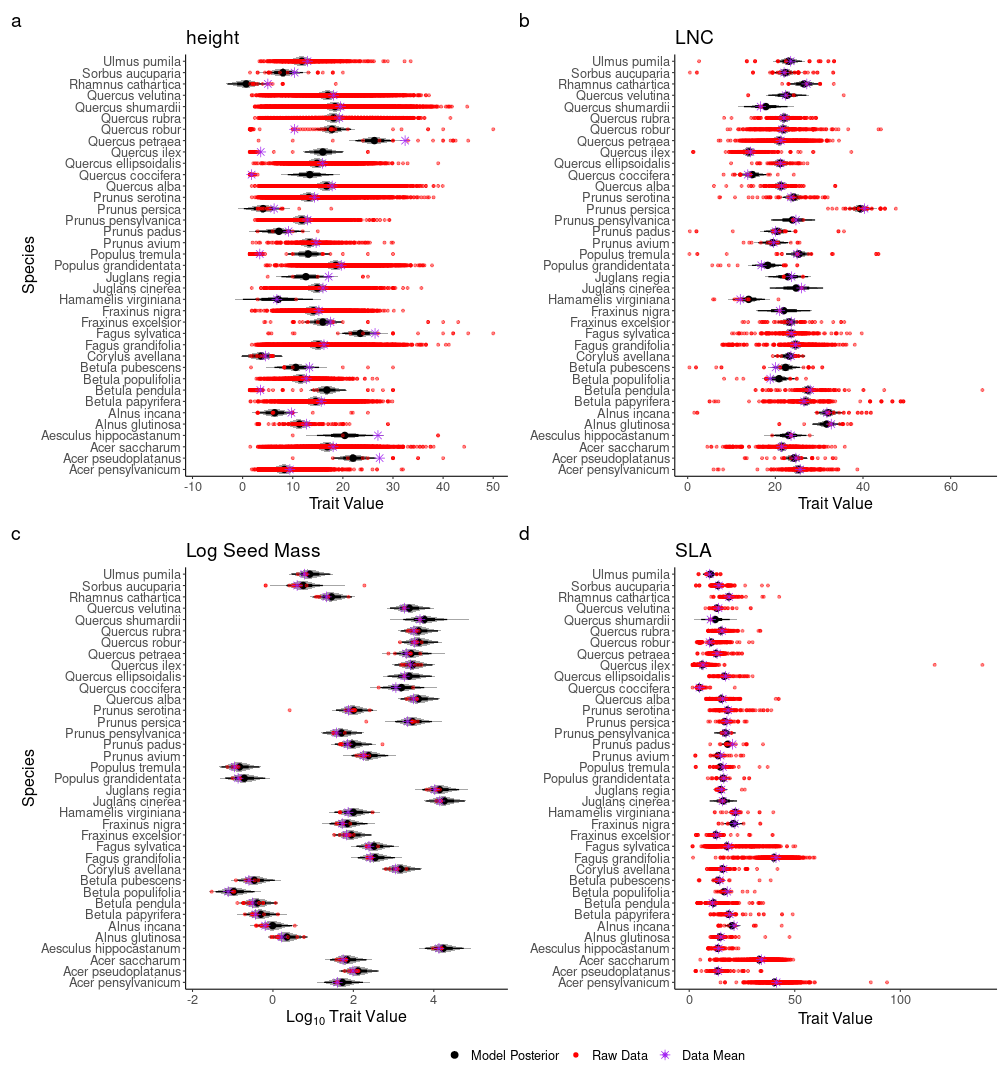
\includegraphics[width=\textwidth]{..//..//analyses/traits/figures/FourTraitFit_37spp.png} 
    \caption{Raw data and posterior esti.}
    \label{figure:TraitDistributions}
\end{figure}

\begin{figure}[h!]
    \centering
 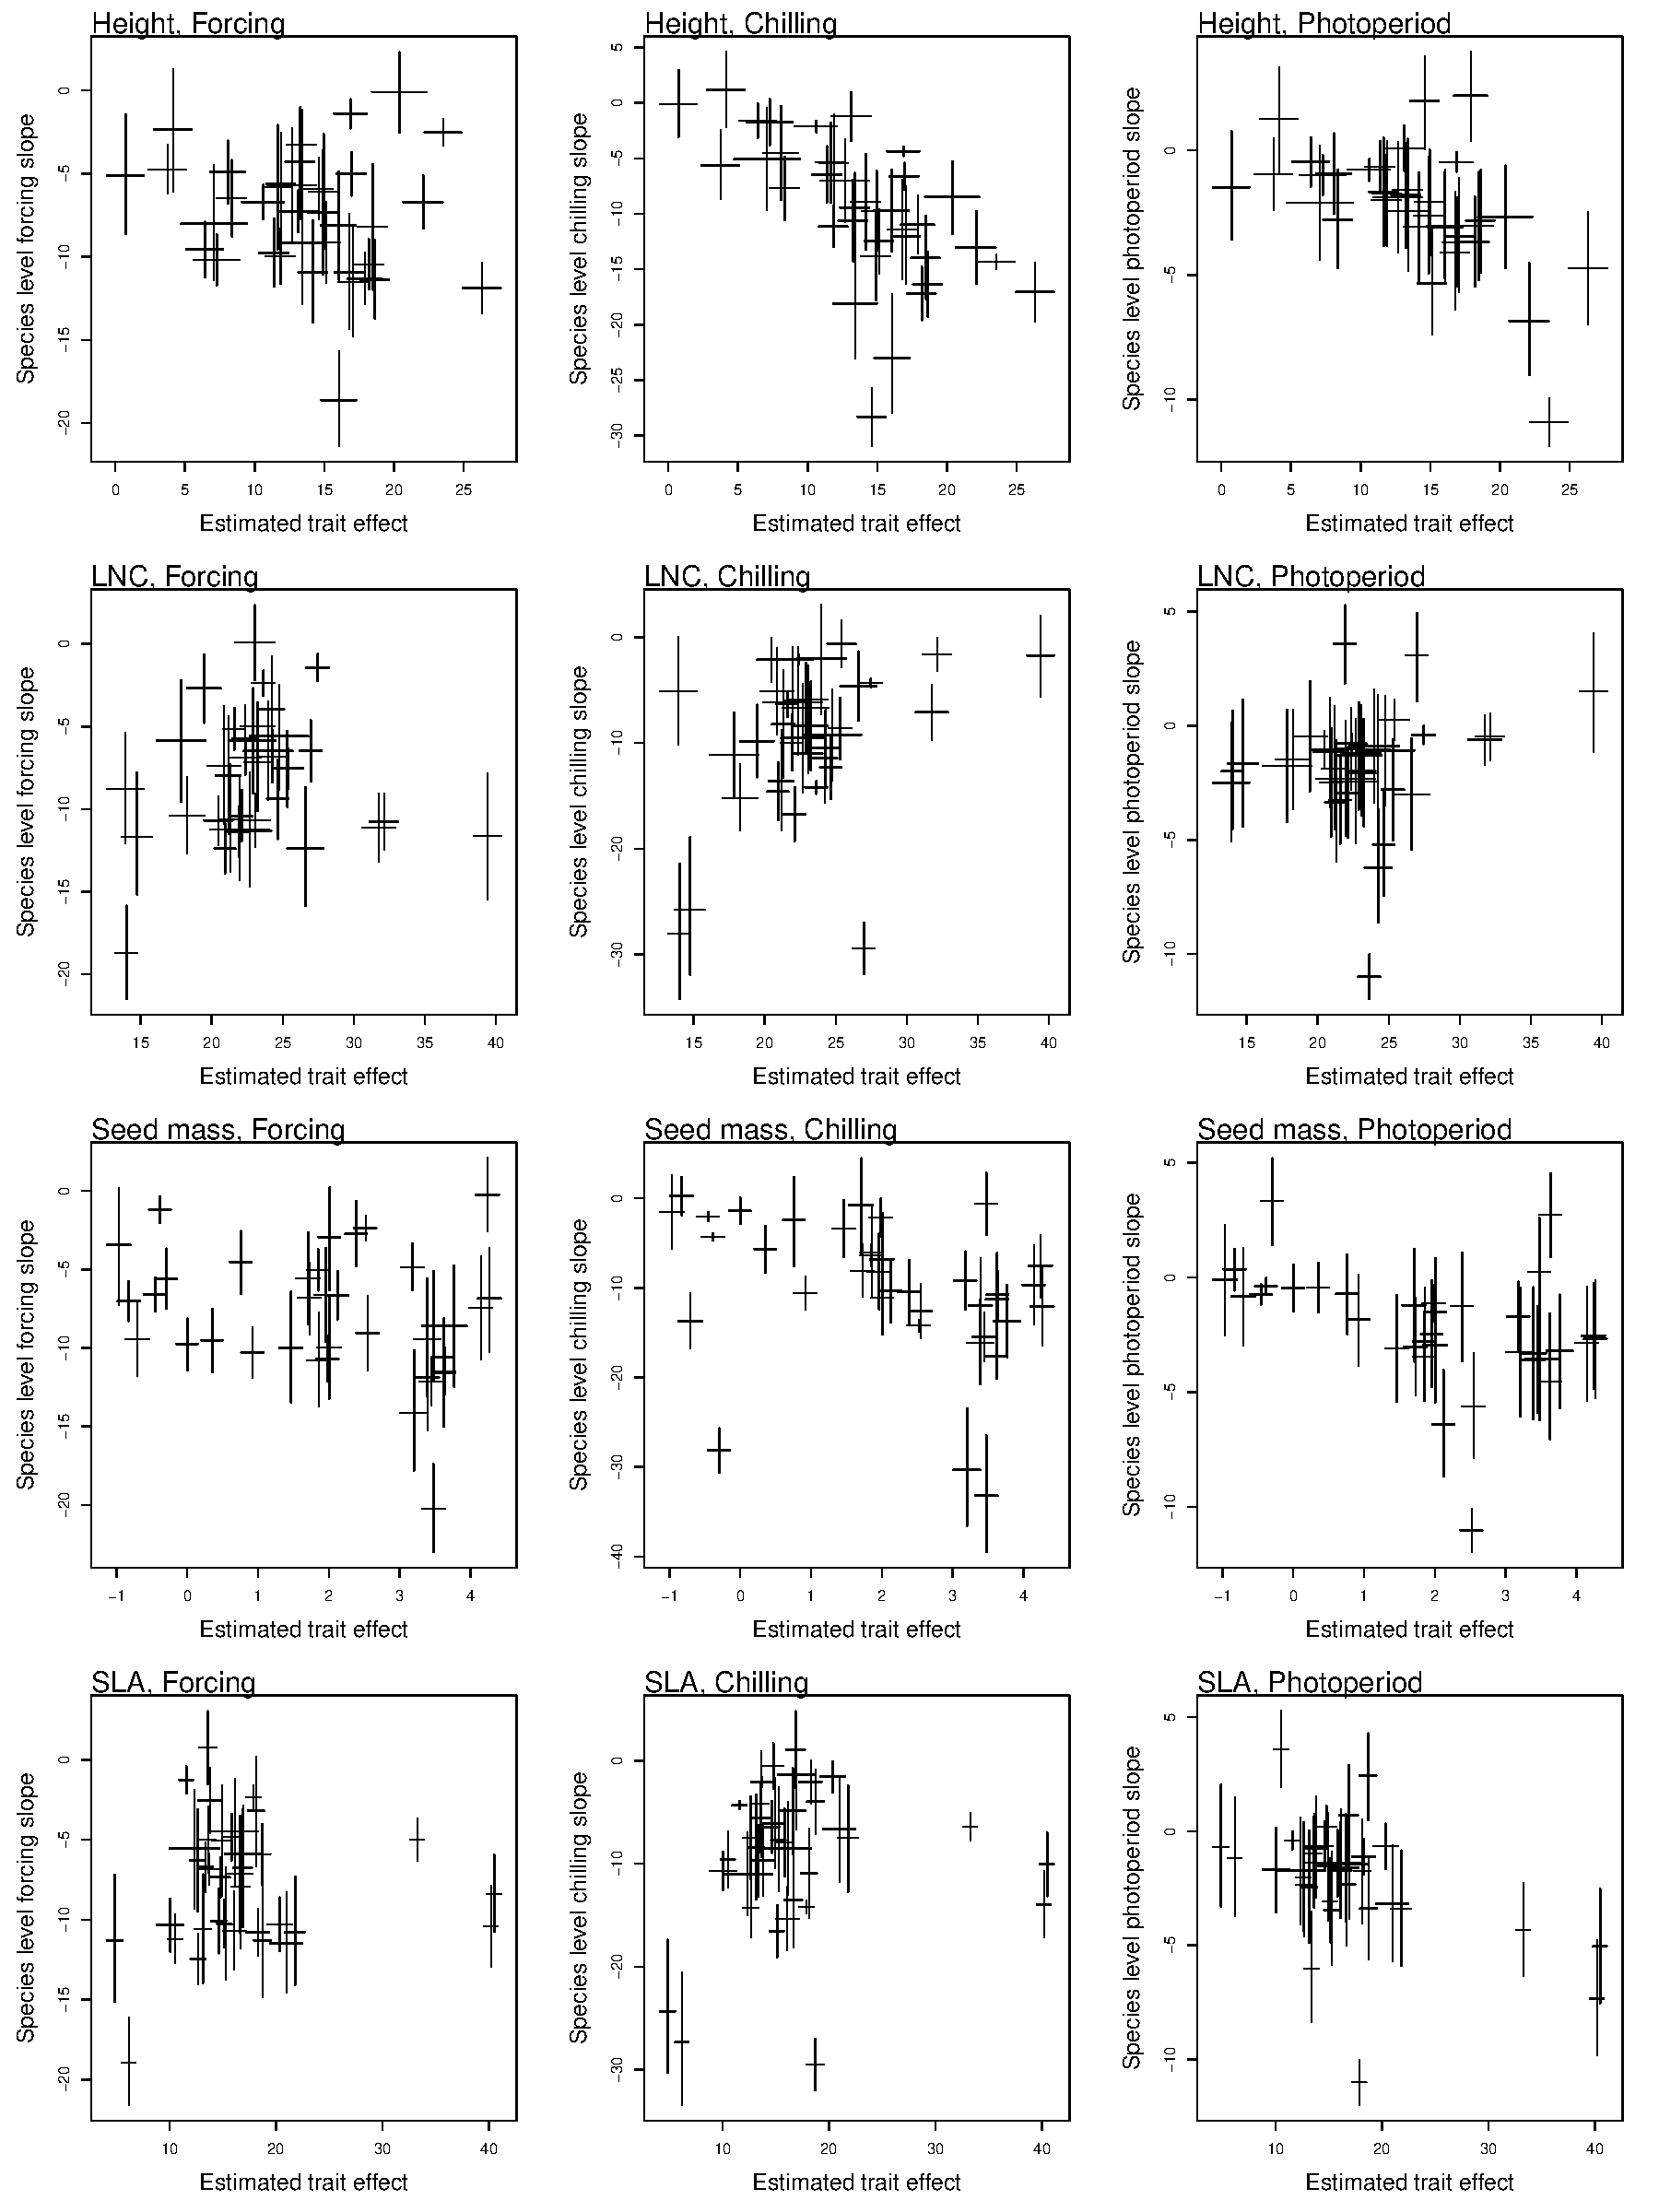
\includegraphics[width=\textwidth]{..//..//analyses/traits/figures/cuetrait.pdf} 
    \caption{Trait relationships with cue slopes}
    \label{fig:cuetraits}
\end{figure}

We found a negative relationship between SLA and each cue response  \ref{fig:cuetraits}, meaning that as SLA increased, responses to each cue became more negative. Chilling was most strongly influenced by SLA (interaction parameter: -9.3: 90\% credible interval: -17.9, -18.1). Species' responses to forcing were also negatively correlated with SLA values ( interaction parameter: -7.8, 90\% credible interval: -14.5, -10.5), as were responses to photoperiod (interaction parameter: -2.0, 90\% credible interval: -11.1, -11.6). For species with high SLA values, such as \textit{Fagus grandifolia}, this negative trait effect produced a more negative slope in the full model relative to the slope when the trait effect is set to zero. The difference in the slopes of species with leaves with low SLA, such as \textit{Quercus ilex}, is much smaller \ref{fig:sla}. The relatively small trait effect of photoperiod is reflected in the smaller difference in the slopes between the full model and the model without the effect of trait \ref{fig:sla}.

The relationship between species height and cue responses was also negative, with increasing tall trees having more negative responses to each cue \ref{fig:cuetraits}. Of the three cues, height had the strongest influence on chilling, with an estimated interaction parameter of -9.6 (90\% credible interval: -14.6, -20.8). The response to forcing was also negative, at -7.5 (90\% credible interval: -12.1, -10.7), as was the photoperiod slope at -2.3 (90\% credible interval: -7.8, -12.4). Tall trees like \textit{Acer pseudoplantanus}, have more negative slopes in the full model compared to models with a zero trait effect, and a much greater difference in their slopes than shorter trees like \textit{Corylus avettana} \ref{fig:slopes}. The trait effect of photoperiod is much smaller, with the slopes of the full model and model without the effect of trait being similar. 

The relationship between LNC and cue responses, was weaker compared to the relationships with other traits, but we still found a negative association between LNC and cue responses \ref{fig:cuetraits}. Chilling was most influenced by LNC (interaction parameter: -9.6 :90\% credible interval: -16, -19.1), followed by the forcing (interaction parameter: -8.1: 90\% credible interval: -12.9, -10.7), while photoperiod had the smallest influence from LNC (interaction parameter: -1.7 :90\% credible interval: -8.2, -12.3). Species like \textit{Alnus glutinosa} that produce leaves with high LNC, the negative trait effect resulted in a more negative slope in the full model relative to the slope of the zero trait effect model. In contrast, species with low LNC like \textit{Quercus ilex} have a much smaller difference in their slopes \ref{fig:slopes}. The model estimated trait effect of LNC for photoperiod is relatively negligible, producing no noticeable differences between the full model and the zero trait effect model  \ref{fig:slopes}. 

Finally, species log seed mass also had a negative relationship with cue responses \ref{fig:cuetraits}. As we observed for other trait models, seed mass had the largest influence on chilling  (interaction parameter: -10: 90\% credible interval: -15.3, -19.4). The influence of seed mass on forcing was also negative, with a slope of -8 (90\% credible interval: -12.2, -10.3), as well as its influence on photoperiod, which had a negative value of -2.2 (90\% credible interval: -7.9, -12.2). The negative trait effect estimated from our model produced more negative slopes, however, given the nature of the log transformation of the seed mass data, the slope of the zero trait effect model is positive. This is shown for the large seeded species \textit{Aesculus hippocastanum} in \ref{fig:slopes}, where here too, the negative effect of the seed mass trait produced a more negative slope in the full model compared to the slope of the model with a zero trait effect \ref{fig:slopes}. The slope differences of small seeded species, like \textit{Alnus glutinosa}, was considerably small. While the estimated trait effect of photoperiod for all species produced more similar slopes for both the full model and the model with a trait effect set to zero \ref{fig:slopes}.
%In line with our our prediction, the high SLA species had earlier budburst dates than the low SLA species.\\

\begin{figure}[h!]
    \centering
 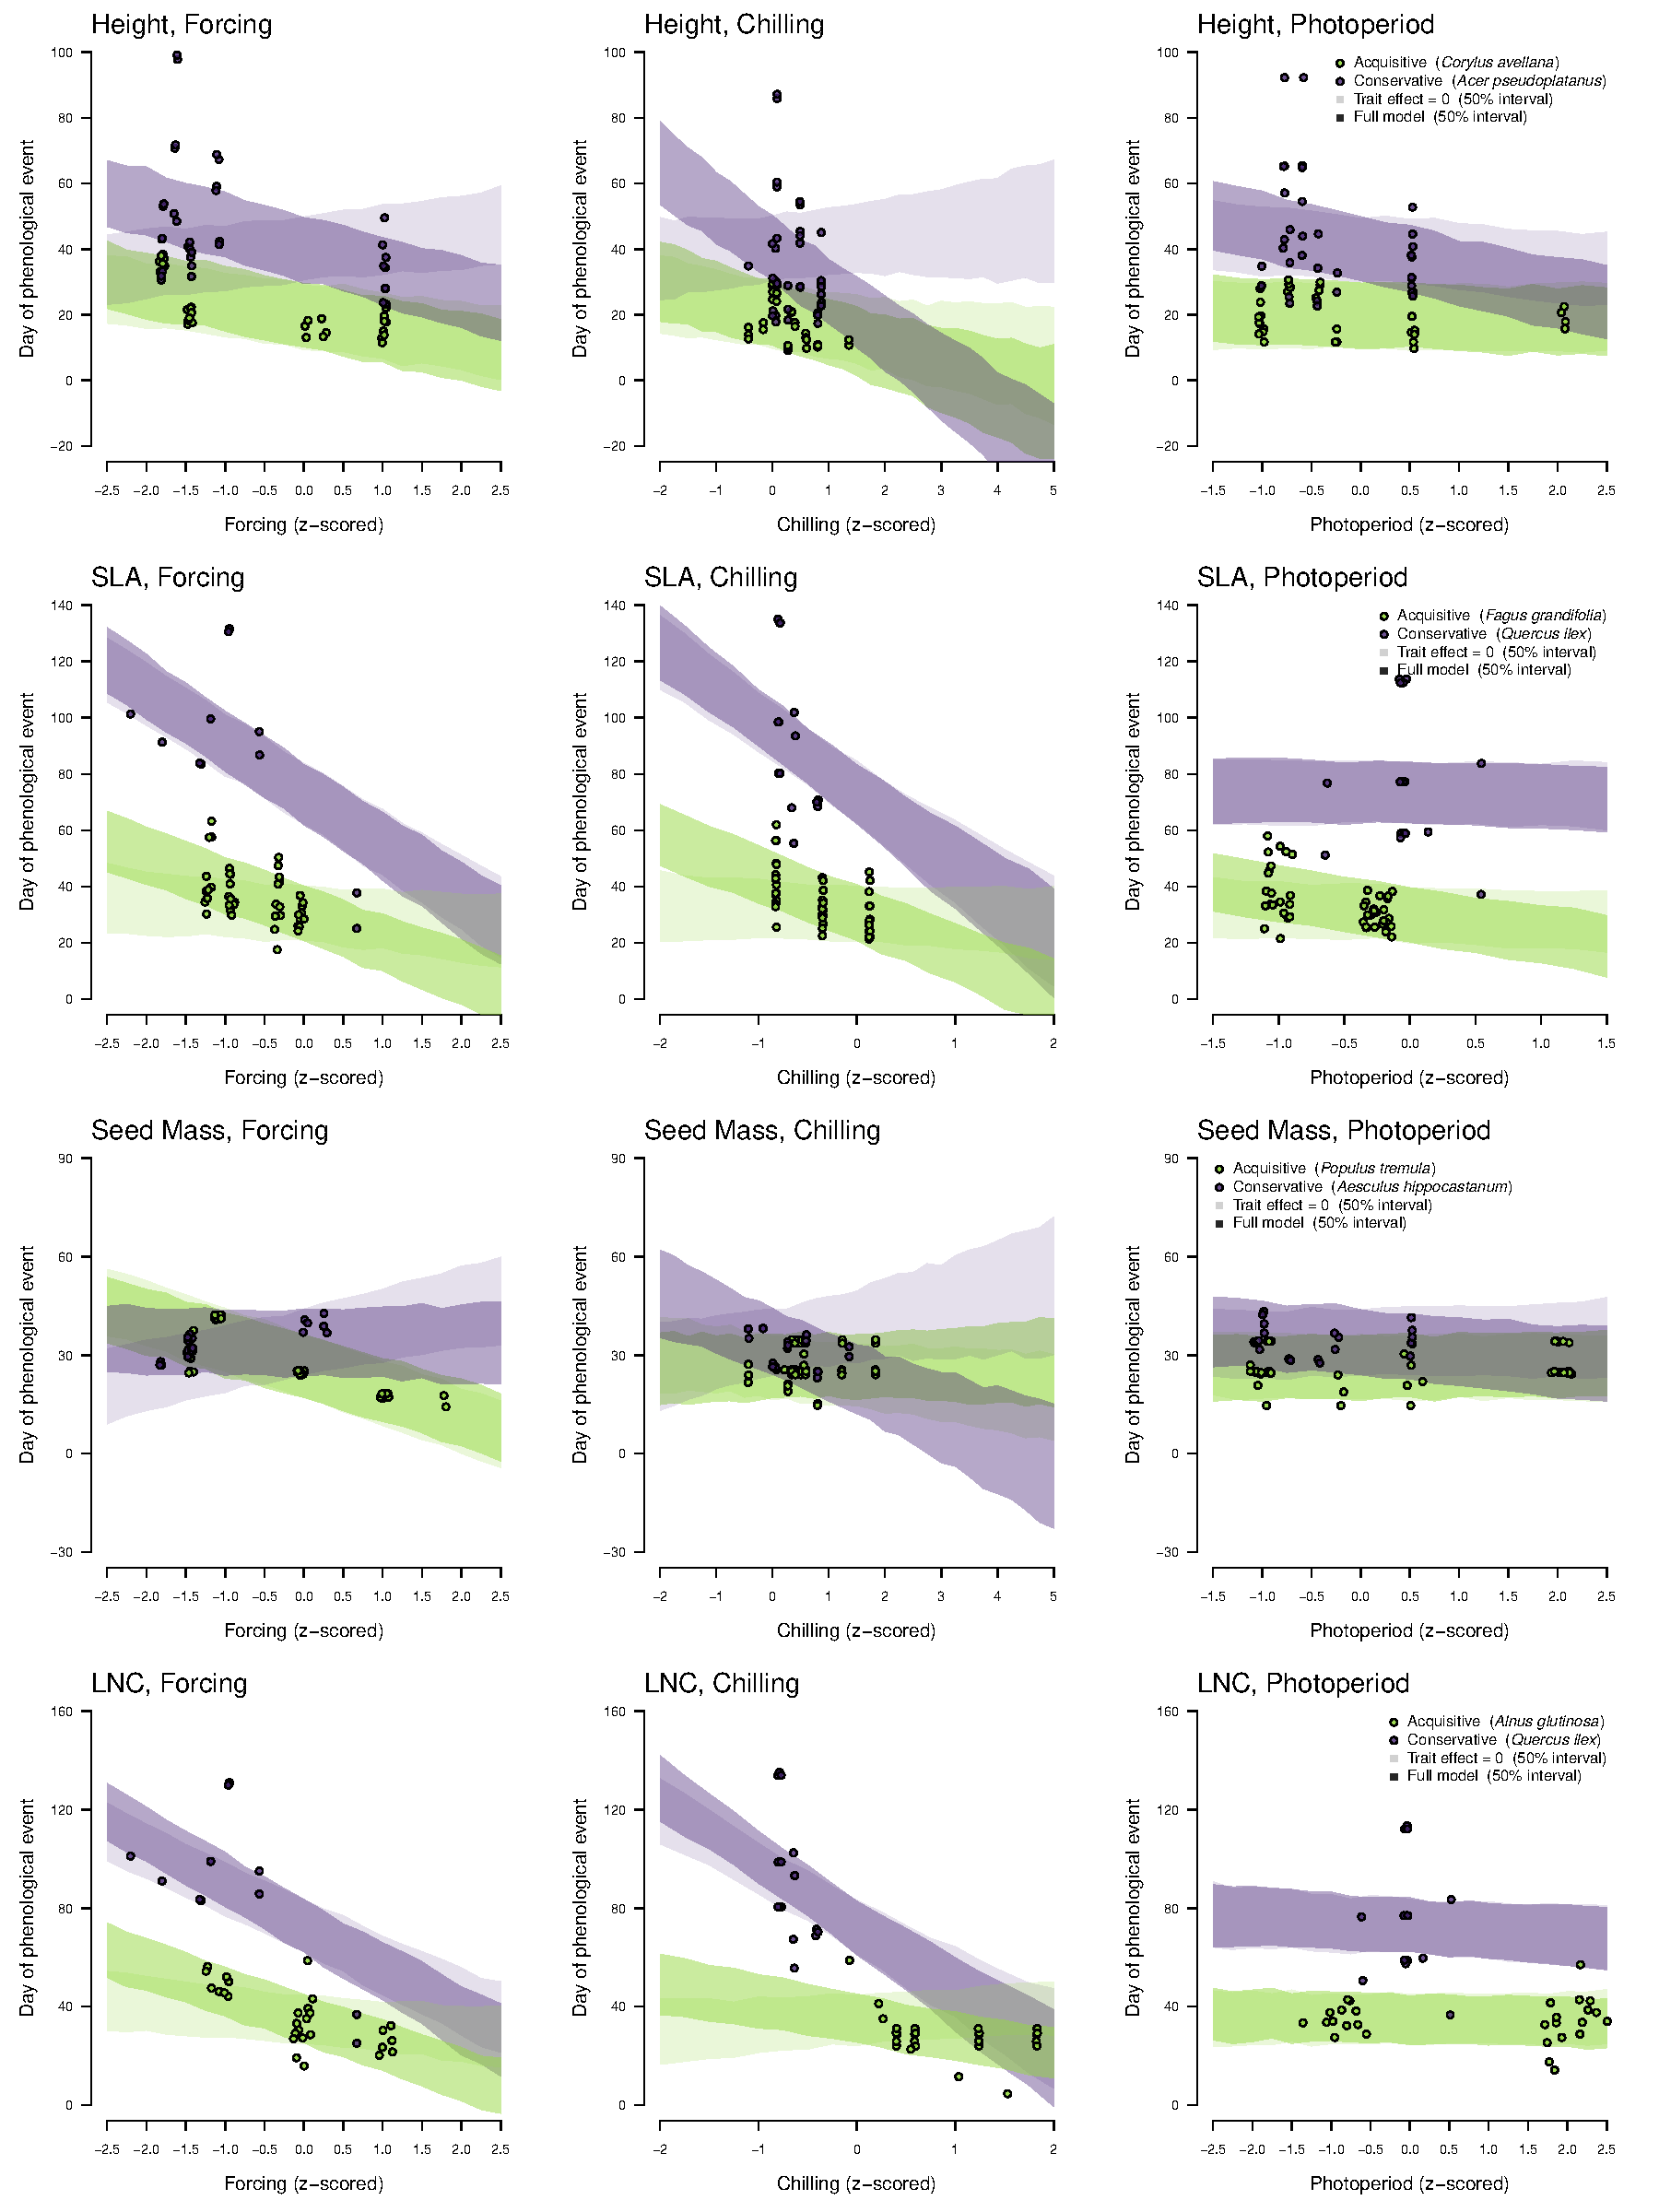
\includegraphics[width=\textwidth]{..//..//analyses/traits/figures/slopesConsAcqu.pdf} 
    \caption{Estimated cue responses for acquisitive and conservative spp.}
    \label{fig:slopes}
\end{figure}

The results of the PGLS analysis suggest there are mostly non-significant phylogenetic relationships between each of our four traits and chilling responses, as well as between hight and forcing, and seed mass and forcing cues (SM tableX). There were no phylogenetic relationships between SLA or LNC and forcing, or for any trait and photoperiod cues (SM tableX). While these results suggest there is some phylogenetic effect influencing the cue response of species for these traits, we were unable to further incorporate these effects into our current analysis given the complexity of our model. 

\section{Discussion}

We found that the functional traits of our assemblage of woody plant species did influence their responses to phenological cues. Overall, our findings suggest that hight trait values shifted phenology more and earlier in response to forcing, chilling, and photoperiod, compared to low trait values. The slopes with species trait responses were in line with our predictions for our structural traits, but not leaf traits. Species that have high trait values for height and seed mass, traits associated with conservative growth strategies, shifted their phenology earlier in response to increases in these three cues. Shorter species with smaller seeds that budburst earlier have lower slopes and lower intercepts, indicating that they require weaker cues to budburst and are less responsive to changes in these cues. However, species with high SLA and LNC, traits we associate with more acquisitive growth, also had negative relationships with cue responses suggesting they too will also advance more with rising cues. High trait values for these leaf traits still advance in response to rising cues, but they do not experience the strong trait effect that we predicted. 

Traits consistently had the largest influence on chilling cues, suggesting they play a role in species avoidance of false spring events or frost tolerance. As we predicted, there were strong negative relationships between chilling cues and height and seed mass \ref{fig:slopes}, indicating that species that are tall and produce large seeds do have greater chilling requirements to budburst and will budburst later in the growing season. This is supported by the identity of species with the largest heights and seed masses, including species in the genus Quercus and \textit{Fagus sylvatica}, which are well known late budbursting species (cite studies showing these species are late). %say something about chilling and leaf traits
 Our model estimates for photoperiod across the four traits also support the findings of previous studies of phenology that observed responses to photoperiod cues to be weakest (citation). To our surprise, the influence of LNC on photoperiod cues was weakest, producing the smallest model estimates. This is a trait most commonly associated with photosynthetic potential and a proxy for the amount of nitrogen rich rubisco enzymes within a leaf. The lack of a relationship therefore suggests that factors other than daylength, such as herbivore pressure, may be selecting for this functional trait.
 
 Our study relating functional traits to phenology is unique from previous research in that we are drawing associations between the traits and the cue responses that define woody species phenologies. In general our model estimates are   


Discuss the DF paper again 

Geoff : "Overall, we found that conservative species, which generally had high traits values for SLA, Height, etc., shifted their phenology more and earlier in response to forcing, chilling, and photoperiod, than acquisitive species with low trait values. This responsiveness is linked to later budbursting - earlier sp have lower slopes bc they require less cues in general, having a lower intercept"

\begin{itemize}
\item What do our results suggest for the relationship between cue use and traits? 
- Species responses to forcing, chilling, and photoperiod cues are influenced by species functional traits. 
- generally in line with previous studies of phenological cues, cue responses were all negative leading to strong advances in bb date 
	\begin{itemize}
	\item Do we find relationships between cues and traits?
	- yes, with the exception of LNC and photoperiod being pretty weak, all traits had an effect of the response of species to cues
	\item Do these trends agree with an acquisitive/conservative tradeoff?
	- yes, species structural traits associated with acquisitive growth strategies did budburst earlier
	- not so much with leaf traits, predicted that high sla and lnc would be earlier, but the slope plots are messier, could be positive for forcing and chilling -- which would be in line with our predictions, but seem to be negative/no trend for photoperiod 
	\end{itemize}
\item How do our results relate to previous studies? 
        Huang et al. 2018 - found several growth strategies - all combinations of early- fast, early-slow, late-fast etc - but looked at flowering
        Osada 2017 - bb later for sp with greater LMA, thickness, Narea – driven by differences across deciduous and evergreen spp; 	Deciduous alone: bb positively correlated with leaf mass, area, vessel diam in cross spp comparisons
\item What do our results suggest for the bigger picture?
Sun, S., D. Jin, and R. Li. 2006. LMA neg correl with leafout; larger LMA = earlier
	\begin{itemize}
	\item How might traits constrain/facilitate future shifts in phenology?
	- our findings do support the idea that phenology is an important functional trait
	\item How might ecosystem functioning shift if species track temperature? How to our results relate to seasonality and frost risk?
	\item What does it mean if more competitive/invasive species respond to warming and start bb earlier - outcompete species and lead to compressed temporal niche?
	\item Relate our results to invasion success 
	\end{itemize}

\item Limitations/strengths?
	\begin{itemize}
	\item we assume stronger cues mean earlier bb but really it's more complicated than this
	\item broad approach means lose detail and compromise - traits come from different populations to the phenology data
	\item disconnect between trait data - observational - and phenology data that is in a controlled environment
	\item limited data may have reduced diversity of traits/strategies - may not be enough to detect predicted trends -- reframe this as less of a limitation and more of a future direction
   \item Why we think mean height values were different from geometric mean values for some species. Talk about the influence of accounting for the study effect. 
	\end{itemize}
\end{itemize}

The trait data used in this experiment was collected independently of the phenological cue experiments, from individuals in diverse ecosystems and community contexts. While this limits our ability to understand the relationships between cue use and traits at the population and individual level, our approach allowed us to test for general trends that scale across populations and can inform future more fine scale research. 

\pagebreak
\bibliographystyle{refs/bibstyles/amnat.bst}% 
\bibliography{refs/traitors.bib}



\end{document}